\section{Single spin}
\subsection{Precession of spin in uniform magnetic field}

We simulate the time evolution of a single spin $\mathbf{S}$ in the presence of a uniform magnetic field $\mathbf{B} = (0,0,B_0)^T$ in the $\mathbf{e}_z$-direction. The components of the spin at equidistant time steps during one period are shown in figure \ref{fig:spin_1}. As expected, we see that the spin precesses around the effective field $\mathbf{H}$, which in this case is given by
\[
	\mathbf{H} = -\pd{H}{\mathbf{S}} = \frac{\partial}{\partial \mathbf{S}}\left( \mu \mathbf{B} \cdot \mathbf{S} \right) =\mu \mathbf{B},
\]
in the absence of damping and anisotropy.

\begin{figure}[htb]
	\centering
	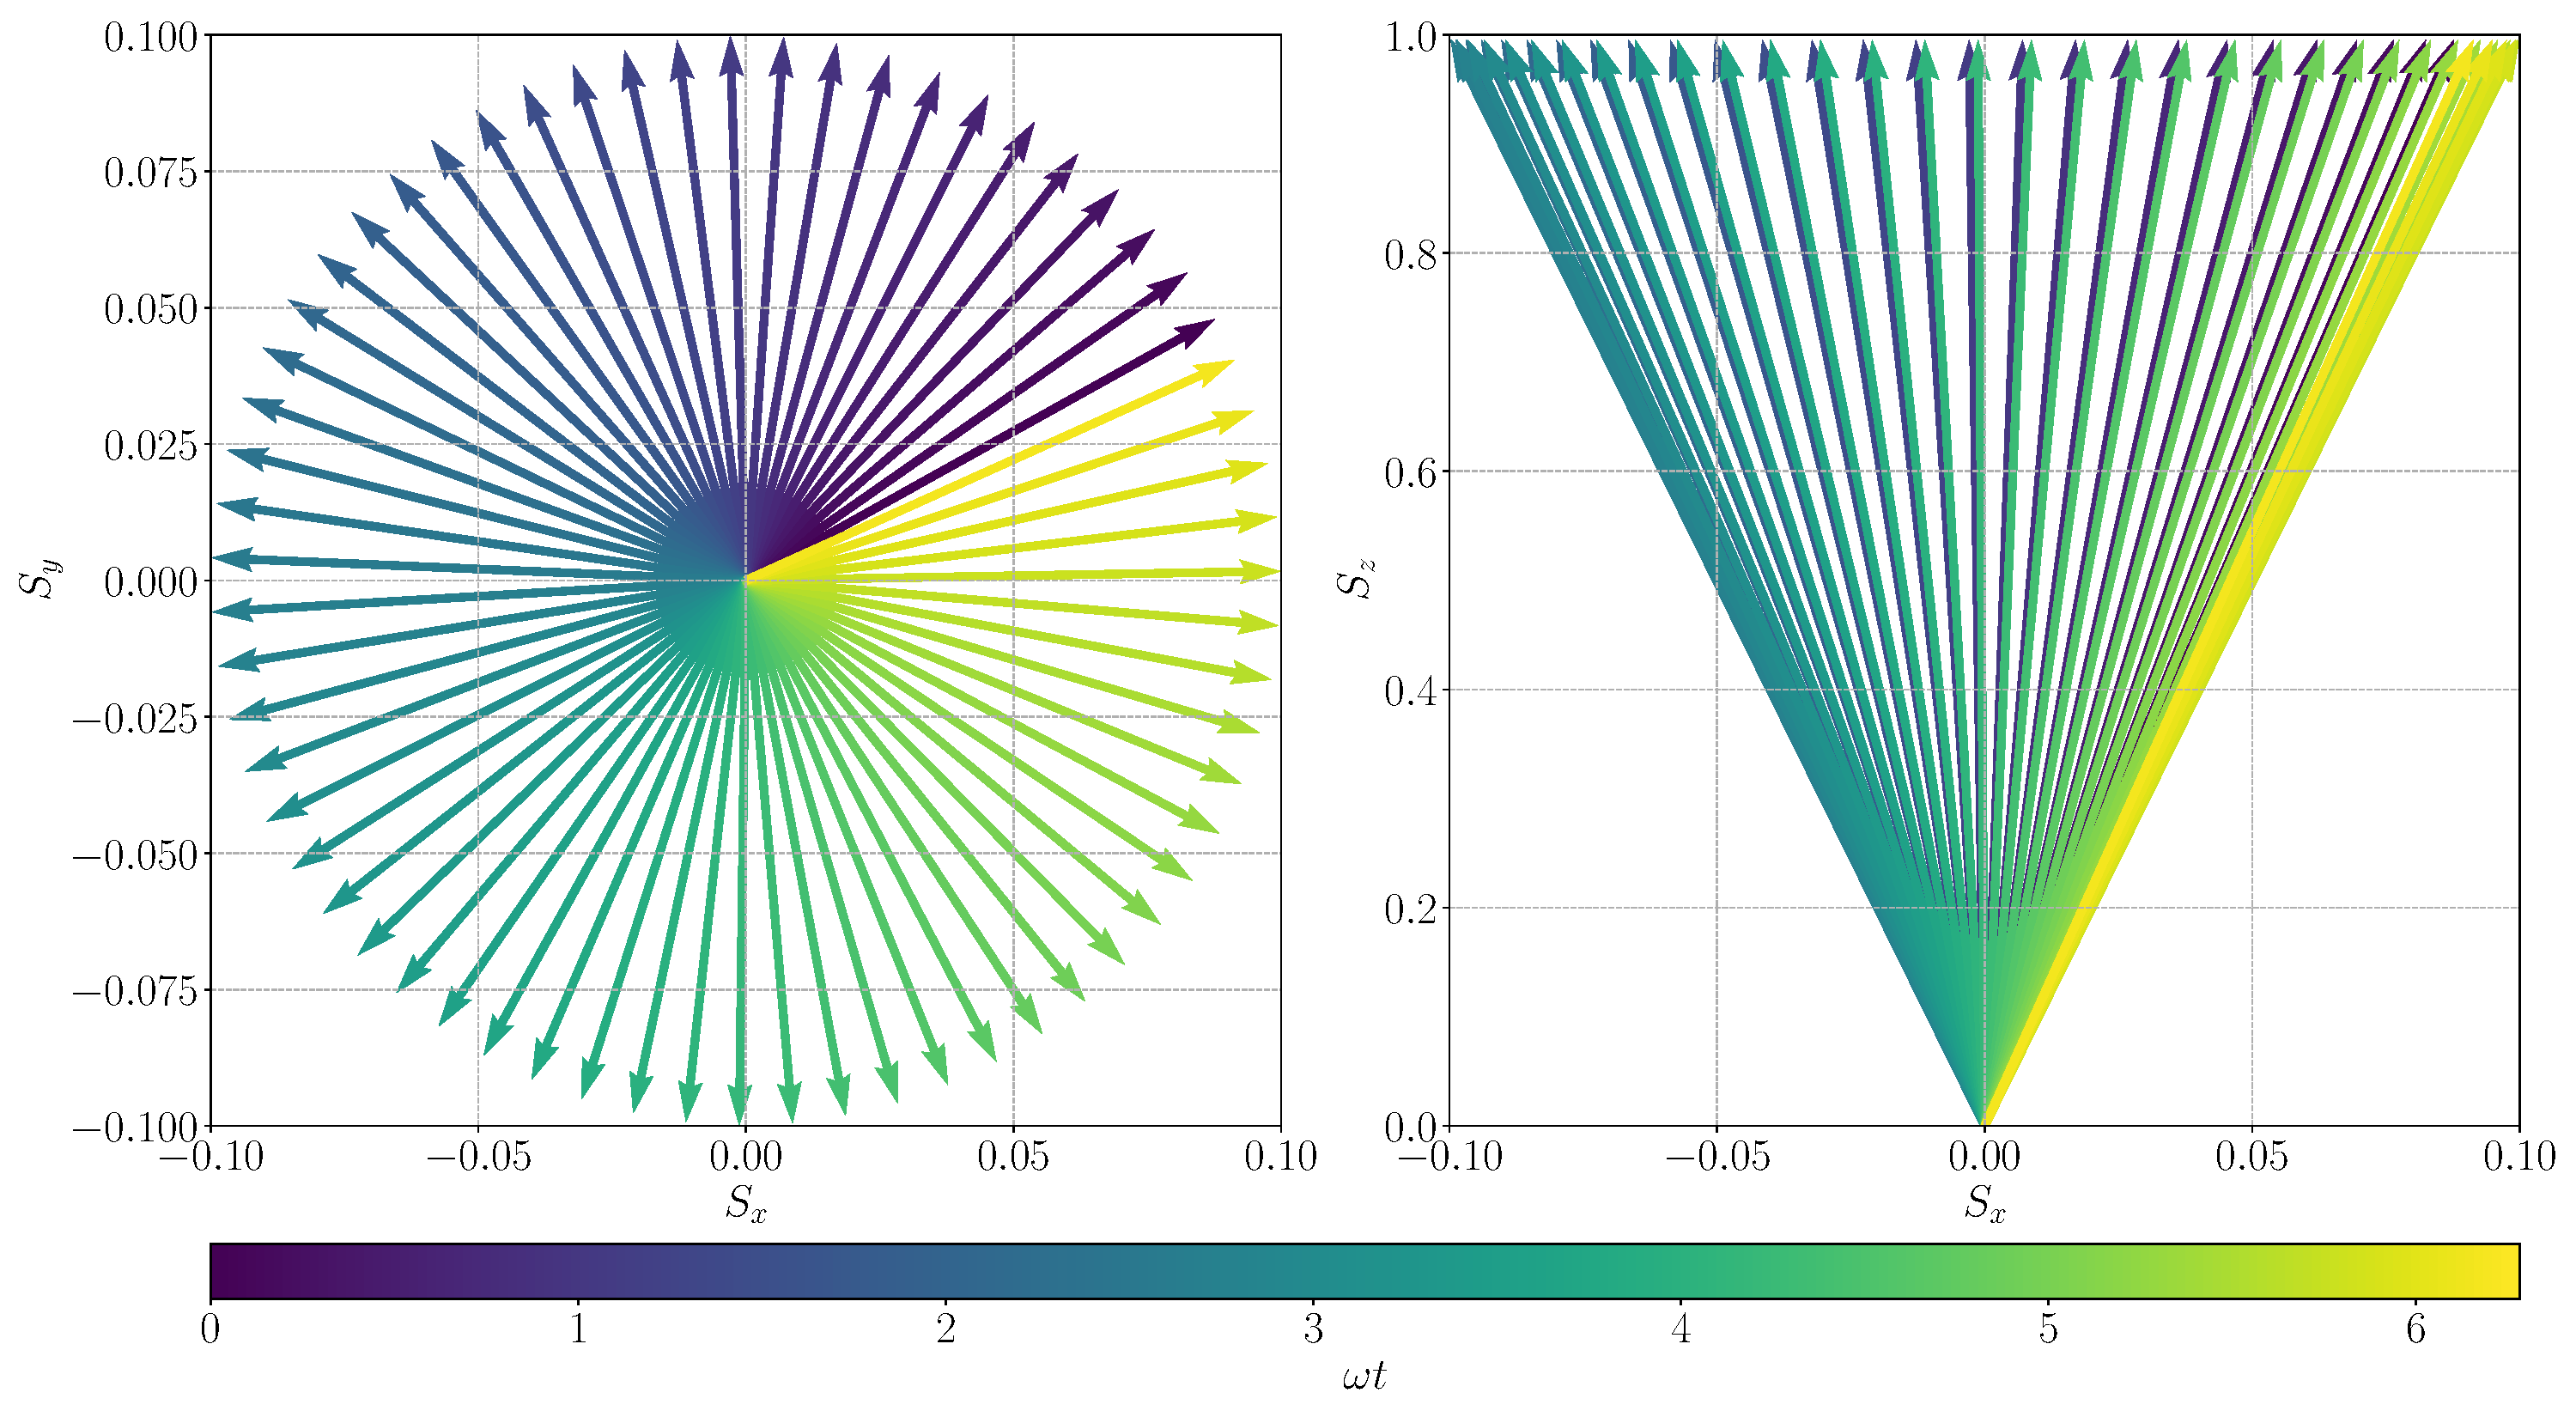
\includegraphics[width=\columnwidth]{../fig/magnet_xy_1}
	\caption{The figure shows the $x$ and $y$ component of the spin during one period in a uniform magnetic field without further interactions.}
	\label{fig:spin_1}
\end{figure}

In this particular case, we can easily find an analytical solution to compare with. The LLG-equation reads
\[
	\partial_t \mathbf{S} = -\gamma \mathbf{S} \times \mathbf{B}.
\]
As $\mathbf{B} = (0,0,B_0)^T$,
\[
	\mathbf{S} \times \mathbf{B} = (S_y \mathbf{e}_x - S_x \mathbf{e}_y) B_0.
\]
Thus, we have two equations 
\begin{equation}\label{eq:eq_sys}
	\begin{cases}
		\partial_t S_x = -\gamma B_0 S_y \\
		\partial_t S_y = \gamma B_0S_x.
	\end{cases}
\end{equation}
which are easily solved by differentiating both with respect to $t$, and then substituting the first order derivatives on the right hand side by the corresponding expressions in \ref{eq:eq_sys}.
\begin{equation}
	\begin{cases}
		\partial^2_t S_x = -\gamma B_0 \partial_t S_y  \\
		\partial^2_t S_y = \gamma B_0 \partial_t S_x.
	\end{cases}
\end{equation}
This yields the two equations
\begin{equation}
	\ddot{S}_x = - \left( \gamma B_0 \right)^2 S_x \quad;\quad \ddot{S}_y = - \left( \gamma B_0 \right)^2 S_y, 
\end{equation}
which have solutions 
\begin{align}
	S_x(t) &= S_x(0) \cos{(\omega t)} - S_y(0) \sin{(\omega t)} \label{eq:exact_1} \\
	S_y(t) &= S_y(0) \cos{(\omega t)} + S_x(0) \sin{(\omega t)} \label{eq:exact_2},
\end{align}

with the frequency $\omega = \gamma B_0$. When comparing the exact solution with the numerical estimate obtained through integrating the LLG-equation with Heun's method, the trajectories of $S_x$ and $S_y$ are as shown in figure \ref{fig:comp}.

%\begin{figure}[htb]
%	\centering
%	\begin{minipage}{0.49\columnwidth}
%	\centering
%	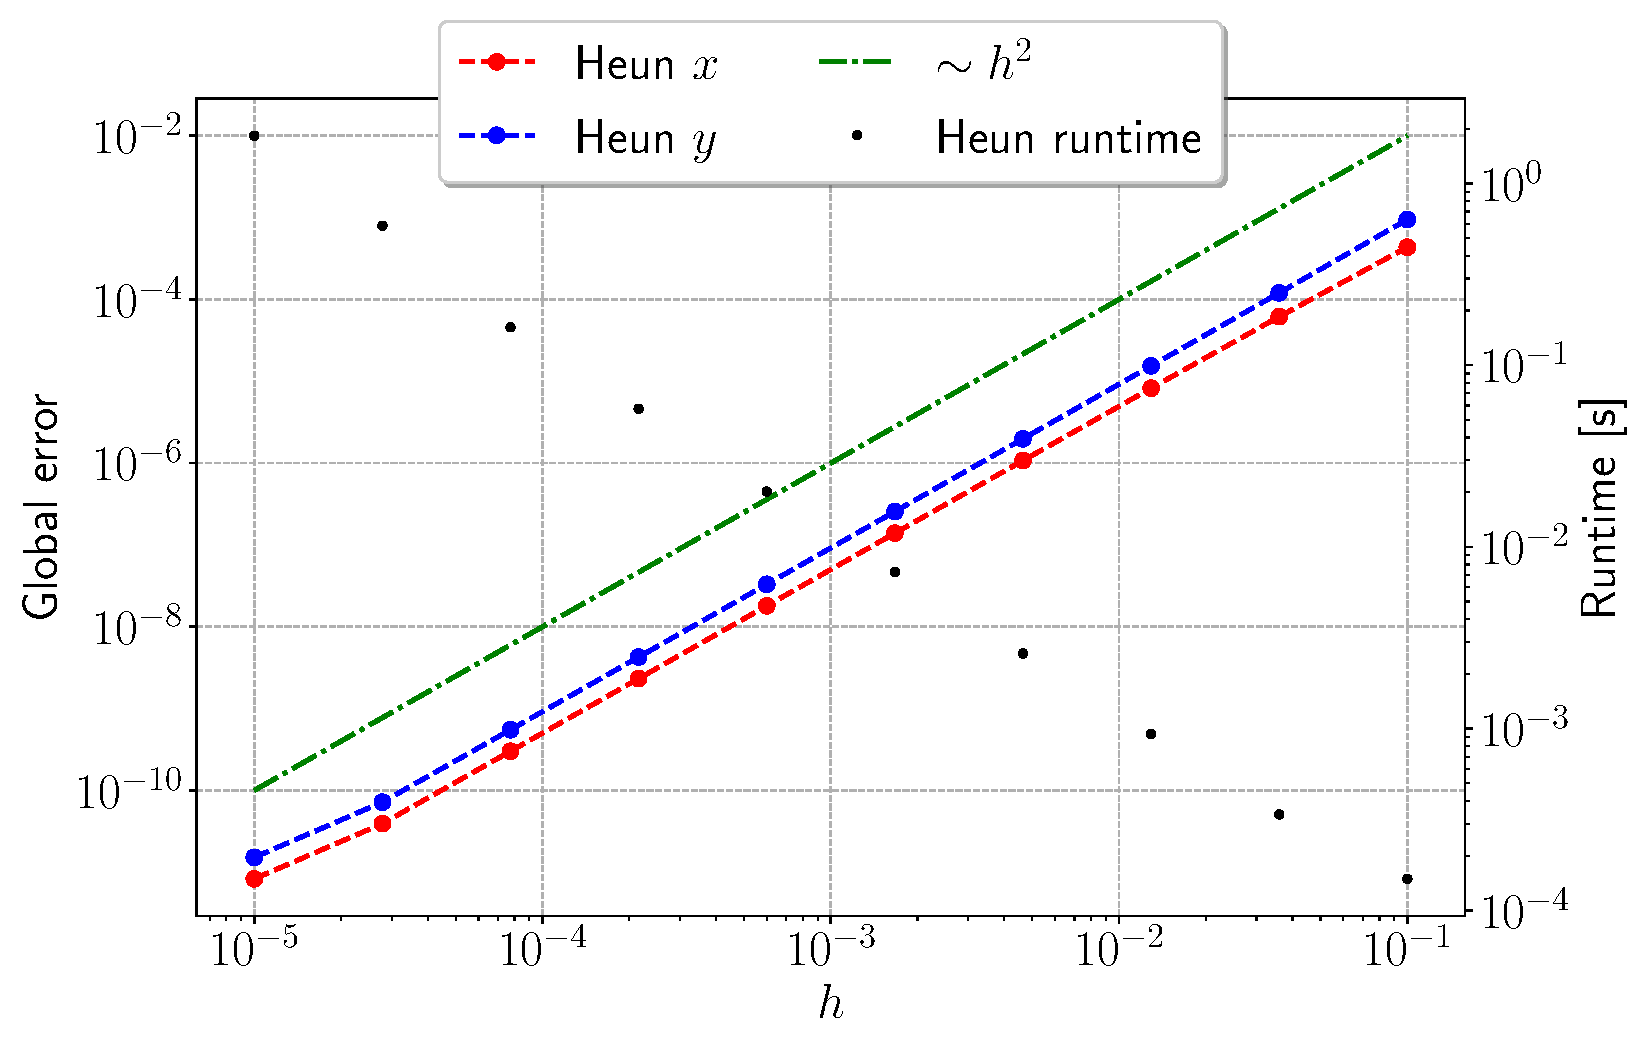
\includegraphics[width =\columnwidth]{../fig/err_heun.pdf}
%	\captionof{figure}{Error as a function of step length for Heun's method.}
%	\label{fig:err_heun}
%	\end{minipage}
%	\hfill
%	\begin{minipage}{0.49\columnwidth}
%	\centering
%	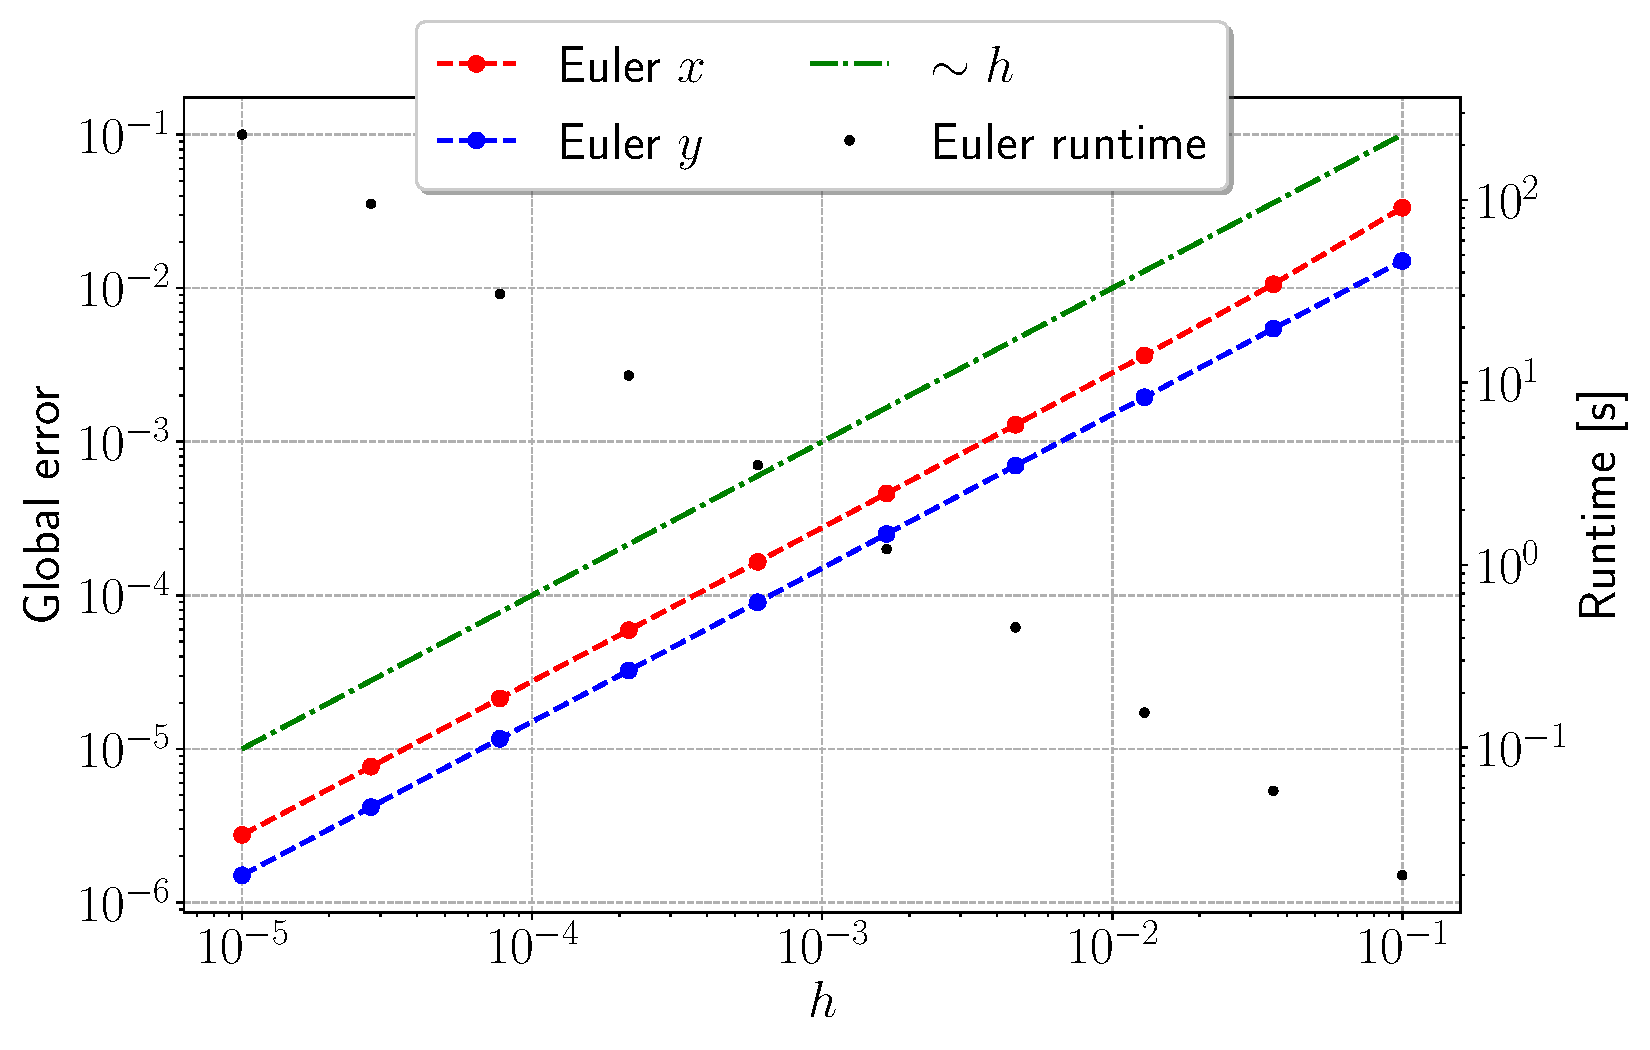
\includegraphics[width = \columnwidth]{../fig/err_euler.pdf}
%	\captionof{figure}{Error as a function of step length for Euler's method.}
%	\label{fig:err_euler}
%	\end{minipage}
%\end{figure}

\begin{figure}[htb]
	\centering
	\begin{minipage}{0.49\columnwidth}
	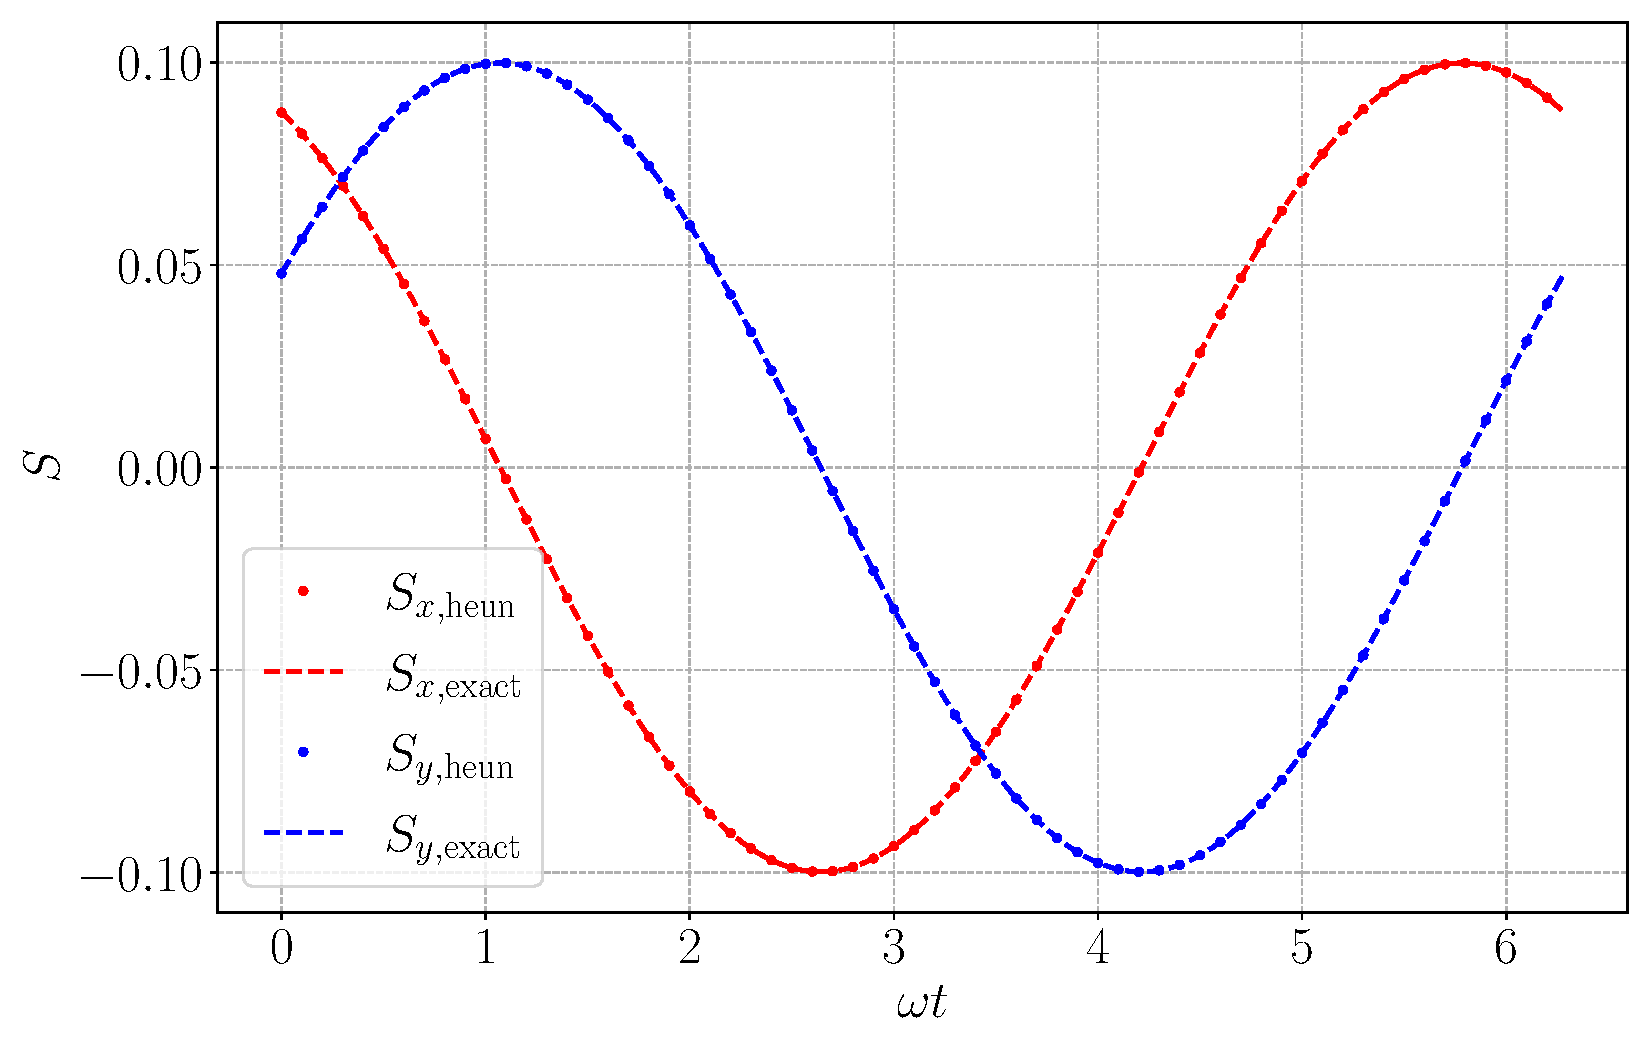
\includegraphics[width=\columnwidth]{../fig/comparison.pdf}
	\captionof{figure}{The plot shows the exact solution given in \eqref{eq:exact_1} and \eqref{eq:exact_2} compared with the numerical solution sampled at every tenth step to be able to distinguish the paths.}
	\label{fig:comp}
	\end{minipage}
	\hfill
	\centering
	\begin{minipage}{0.49\columnwidth}
	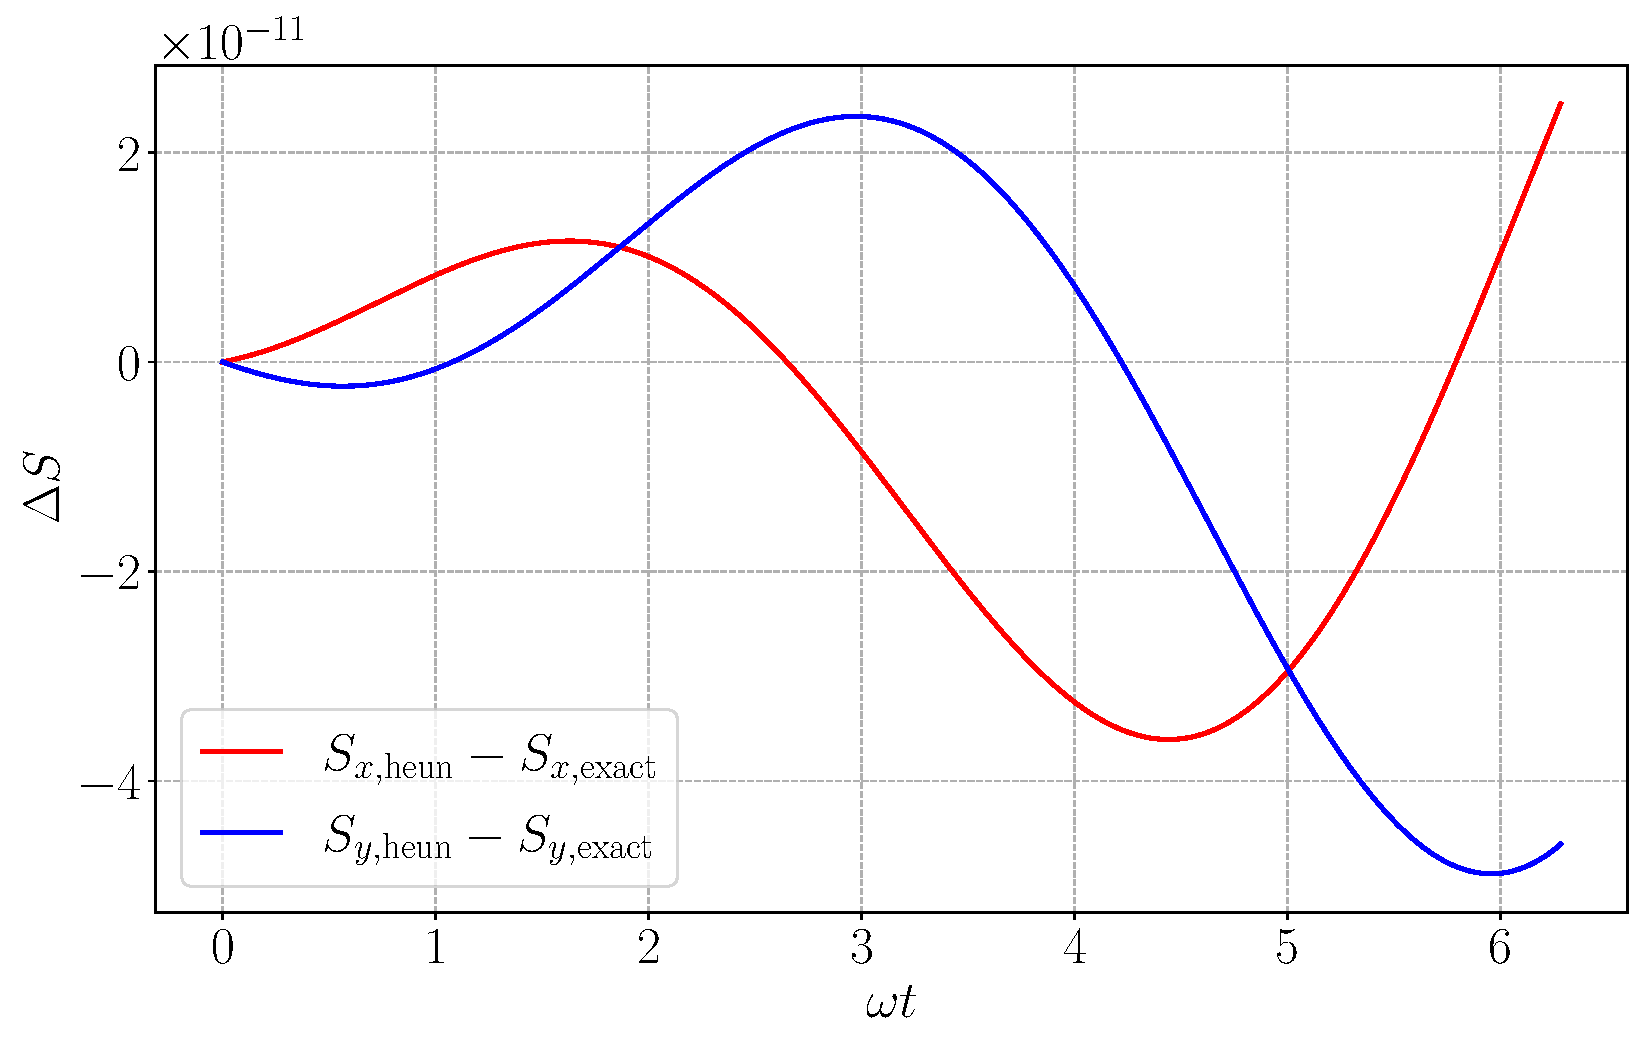
\includegraphics[width=\columnwidth]{../fig/comparison_diff.pdf}
	\caption{The plot shows the difference between the exact solutions given in \eqref{eq:exact_1} and \eqref{eq:exact_2}, and the numerical solutions over one period.}
	\label{fig:comp_diff}
	\end{minipage}
\end{figure} 
It is perhaps more enlightening to consider the pointwise difference of the exact and numerical solution. This is shown in figure \ref{fig:comp_diff}. The figure shows that the deviations locally oscillate, and that the absolute global deviations increase with time as we'd expect. Further considerations on the deviations are considered in \ref{sec:error}.


\subsection{Error analysis}\label{sec:error}

For the error analysis, I choose $10$ logarithmically spaced step-lengths from $10^{-5}$ to $10^{-1}$. As a measure of the \textit{global error}, that is the cumulated error over one period. The error as a function of step length is shown in figure \ref{fig:err_heun}.
\begin{figure}[htb]
		\centering
		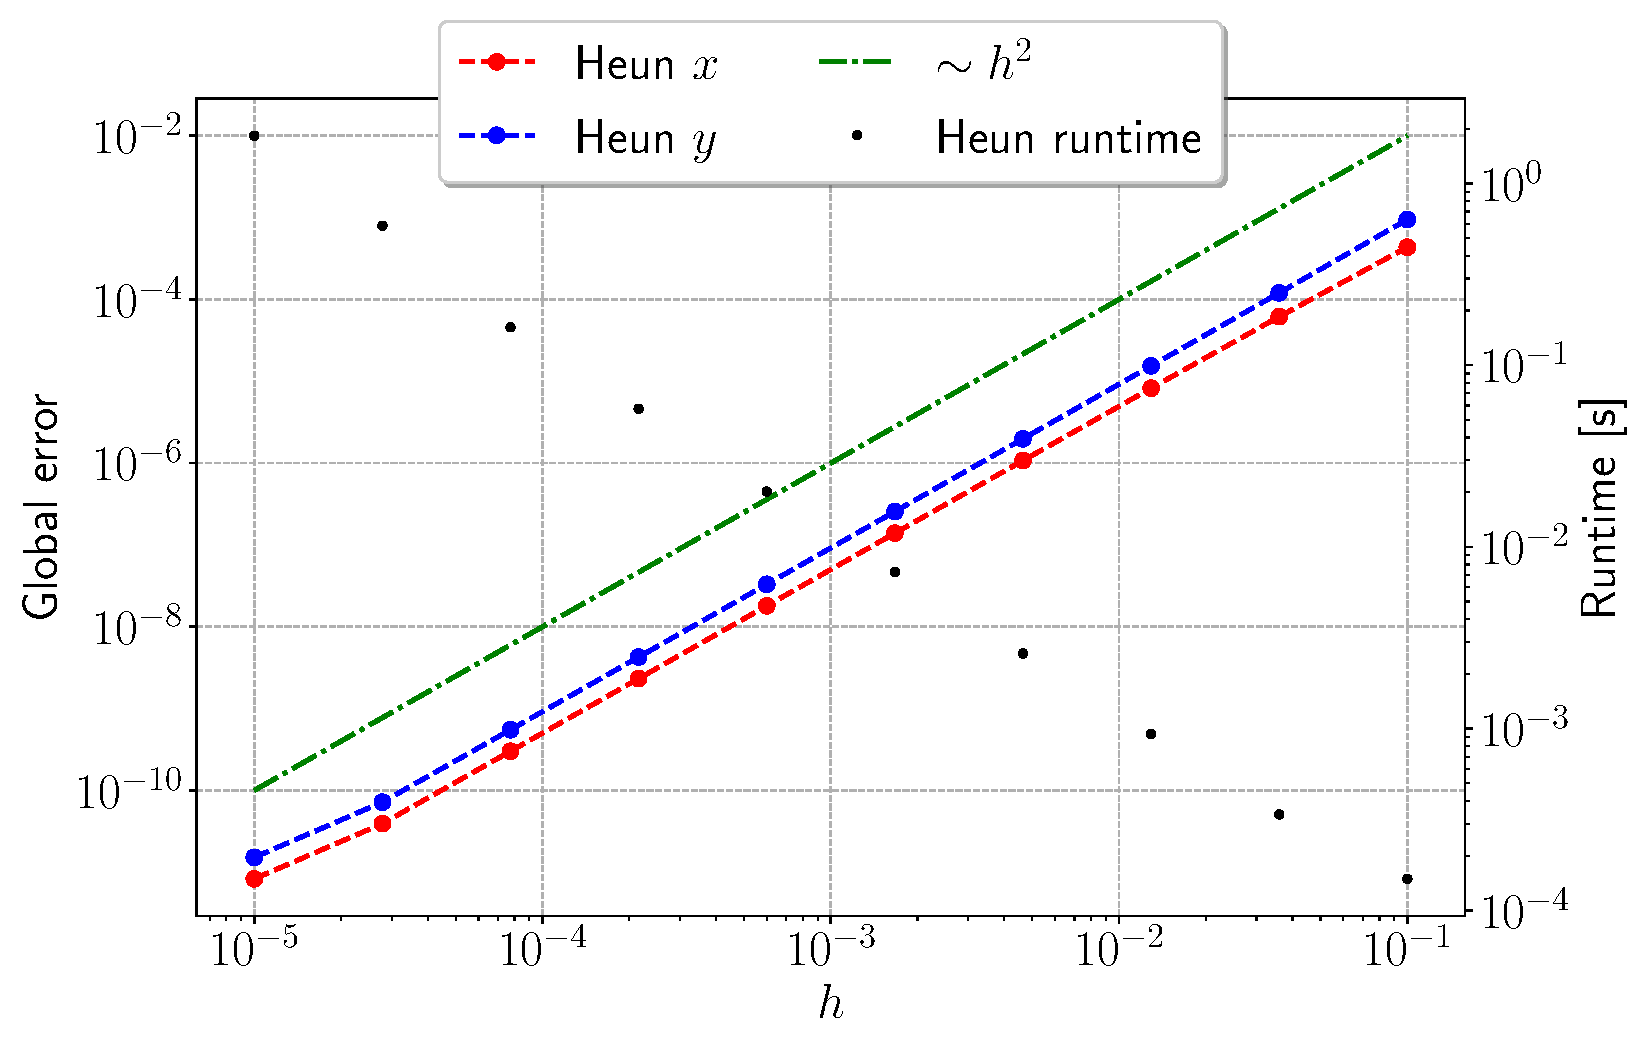
\includegraphics[width =0.8\columnwidth]{../fig/err_heun.pdf}
		\caption{Error as a function of step length for Heun's method.}
		\label{fig:err_heun}
\end{figure}
%\begin{figure}[htb]
%	\centering
%	\begin{minipage}{0.49\columnwidth}
%	\centering
%	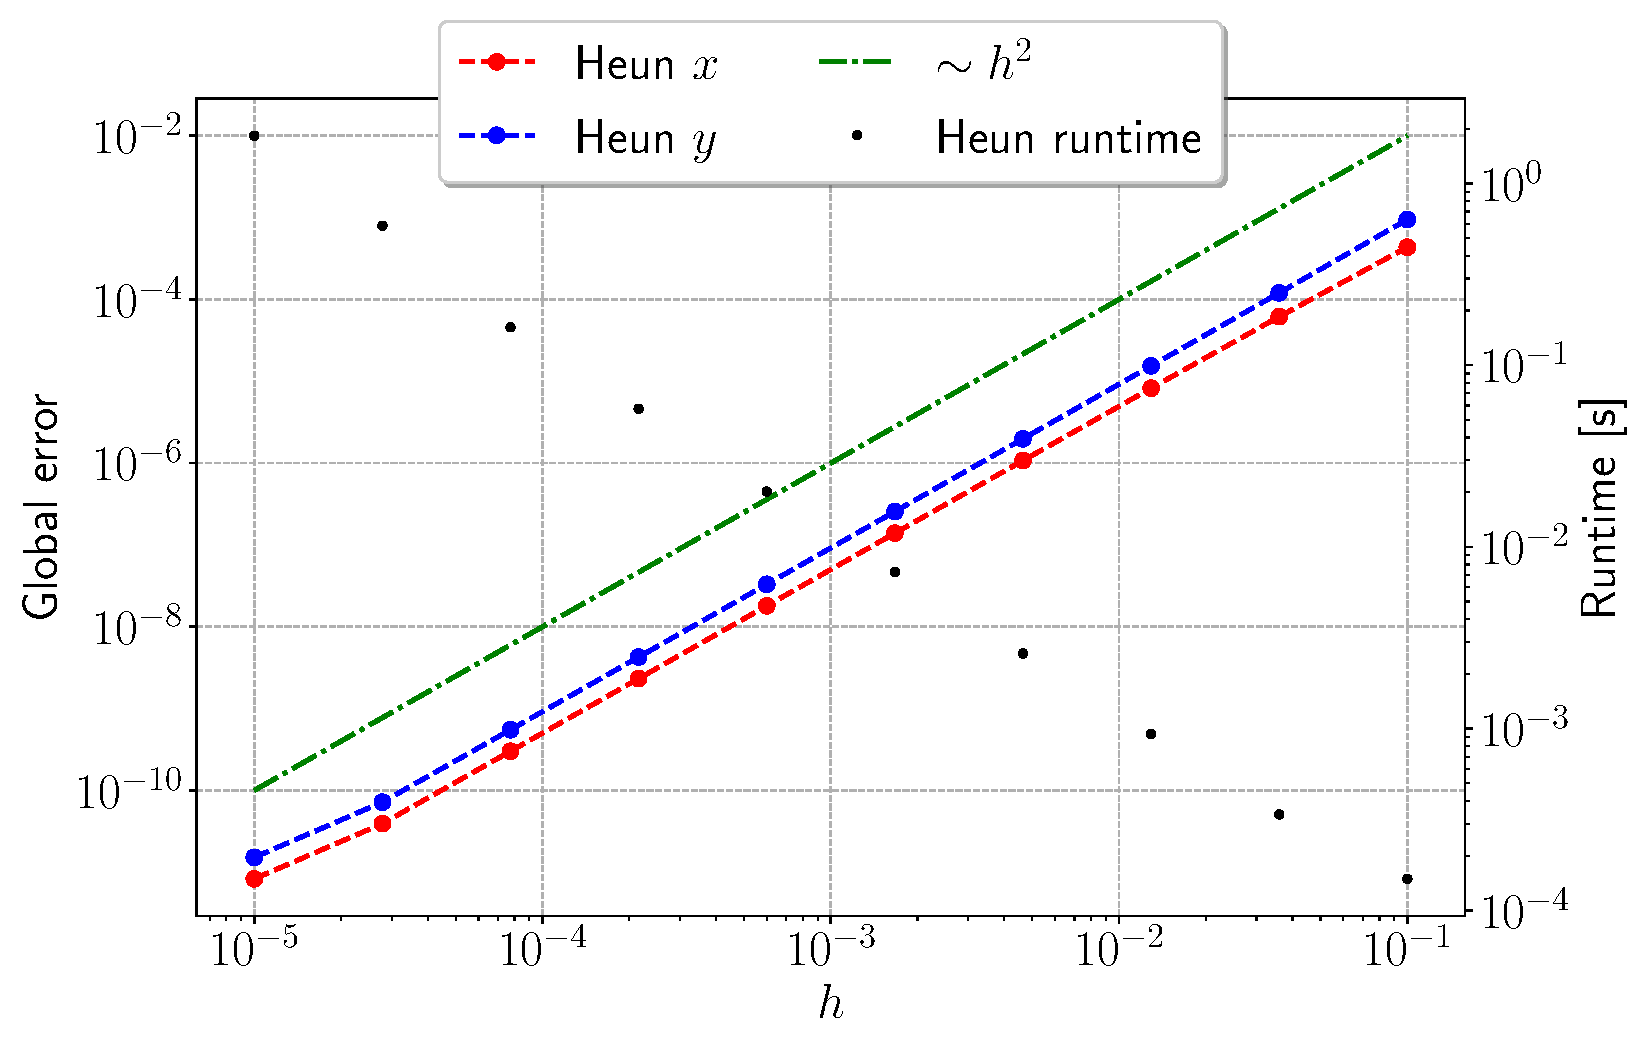
\includegraphics[width =\columnwidth]{../fig/err_heun.pdf}
%	\captionof{figure}{Error as a function of step length for Heun's method.}
%	\label{fig:err_heun}
%	\end{minipage}
%	\hfill
%	\begin{minipage}{0.49\columnwidth}
%	\centering
%	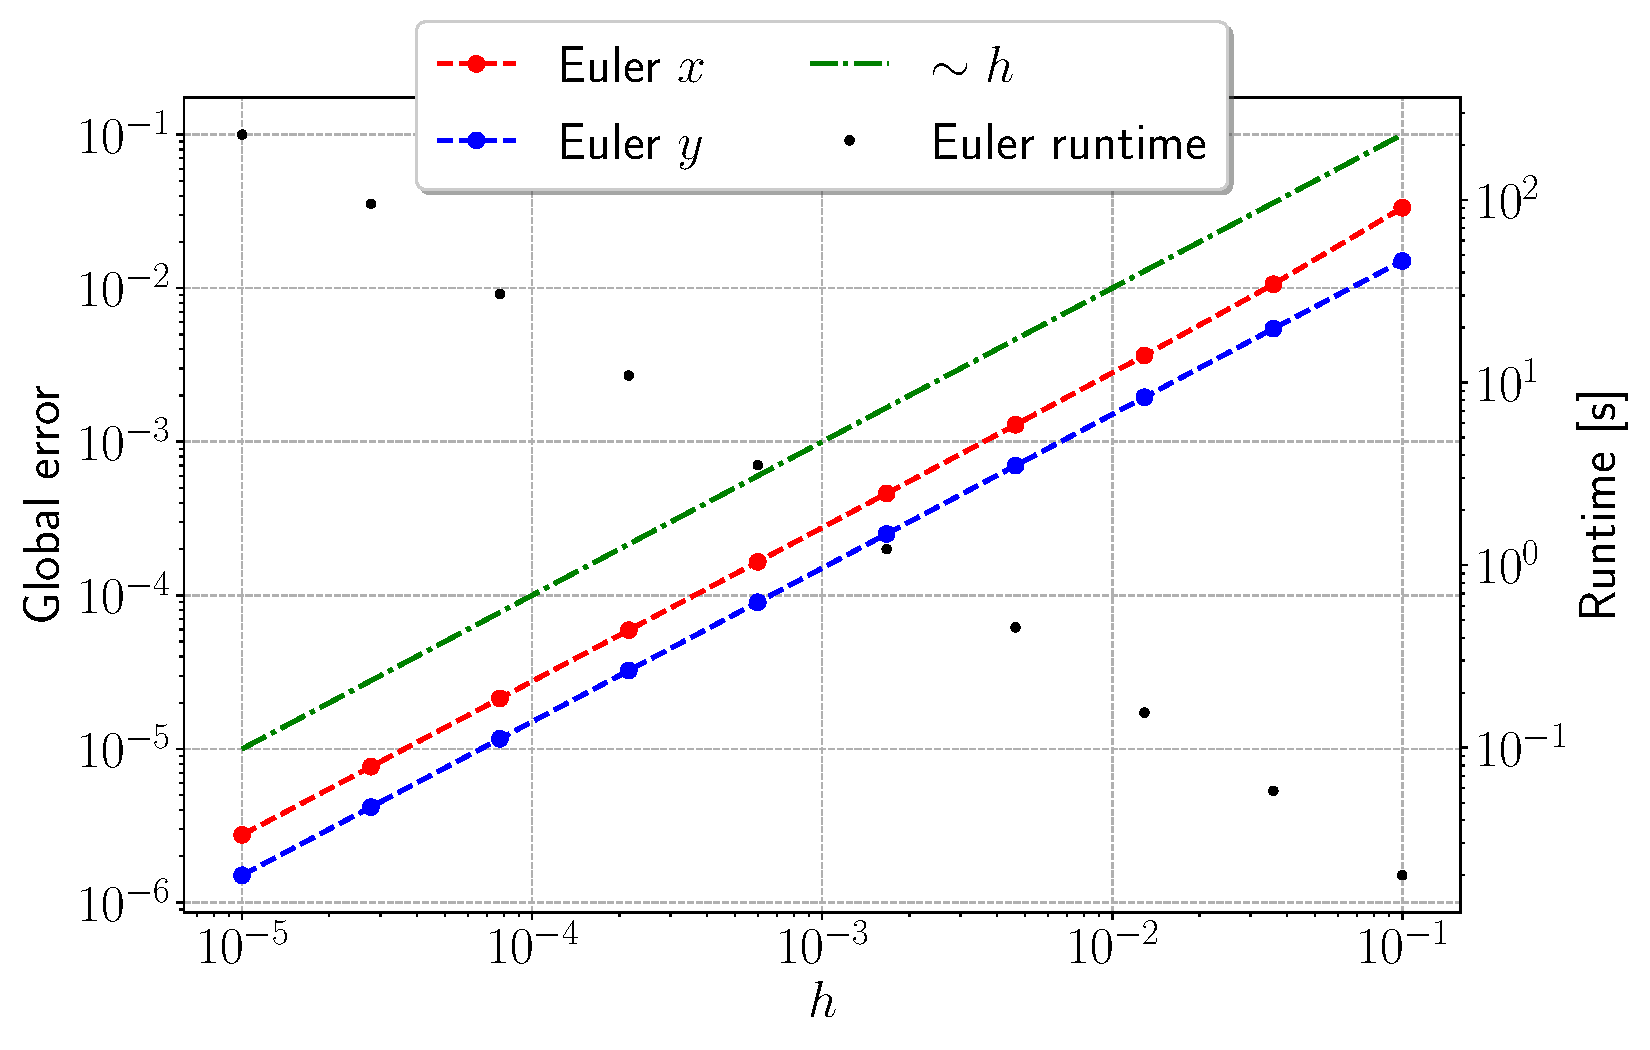
\includegraphics[width = \columnwidth]{../fig/err_euler.pdf}
%	\captionof{figure}{Error as a function of step length for Euler's method.}
%	\label{fig:err_euler}
%	\end{minipage}
%\end{figure}
Since Heun's method is of second order, we would expect its slope in a log-log plot to be roughly $2$. Comparing to the line $\sim h^2$ shows that this is the case, at least for reasonably large $h$. In figure \ref{fig:err_heun} we notice that the error line seems to have a kink for very low step lengths. This can be understood by the fact that the round-off error done by the machine pollutes the numerical calculation. As a rough estimate of the pollution: for $h = 1\cdot 10^{-5}$ we do roughly $60\,000$ steps on one period. If the round-off error in each step is $\approx 10^{-15}$ we would expect an accumulated error of $\approx 6\cdot 10^{-11}$, which indeed is comparable to the error at $h = 10^{-5}$ in figure \ref{fig:err_heun}. This accounts for the kink in the error at $h=10^{-5}$.  

In figure \ref{fig:err_euler} we have plotted the errors for Euler's method for the same step lengths. This plot clearly demonstrates the well known fact that Euler's method is of order $1$. Notice that the error never becomes so small as to be affected by numerical round-off error done by the machine.

\begin{figure}[htb]
	\centering
	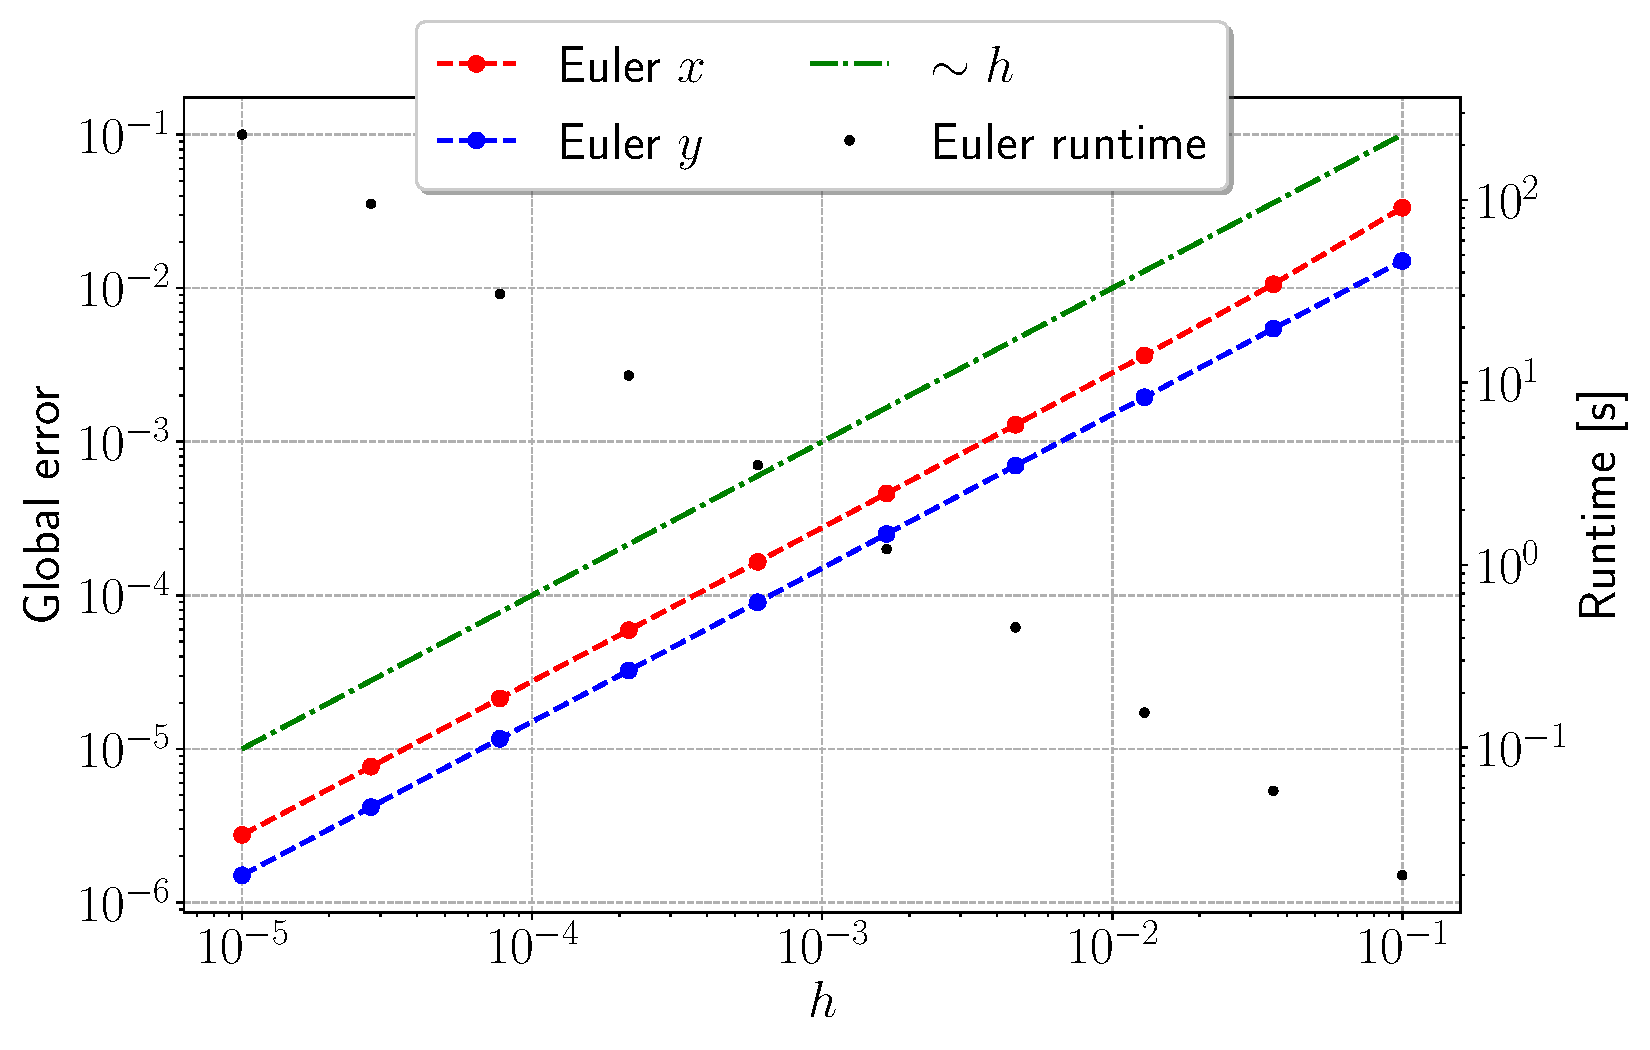
\includegraphics[width =0.8\columnwidth]{../fig/err_euler.pdf}
	\caption{Error as a function of step length for Euler's method.}
	\label{fig:err_euler}
\end{figure}

\subsection{Damped precession of spin in magnetic field}

Next, we include damping in the model. This amounts to setting $\alpha \neq 0$. The plots of the trajectories in the $x$ and $y$ direction for three different damped cases is shown in figure \ref{fig:damped}. The damping lifetime $\tau =  \frac{1}{\alpha \omega}$ is fitted to the plots by plotting 
\[
	\pm \sqrt{S_x^2 + S_y^2} \exp{\left(-\alpha \omega t\right)},
\]
which is approximately the shape of the envelope in the presence of damping.  

\begin{figure}[htb]
	\centering
	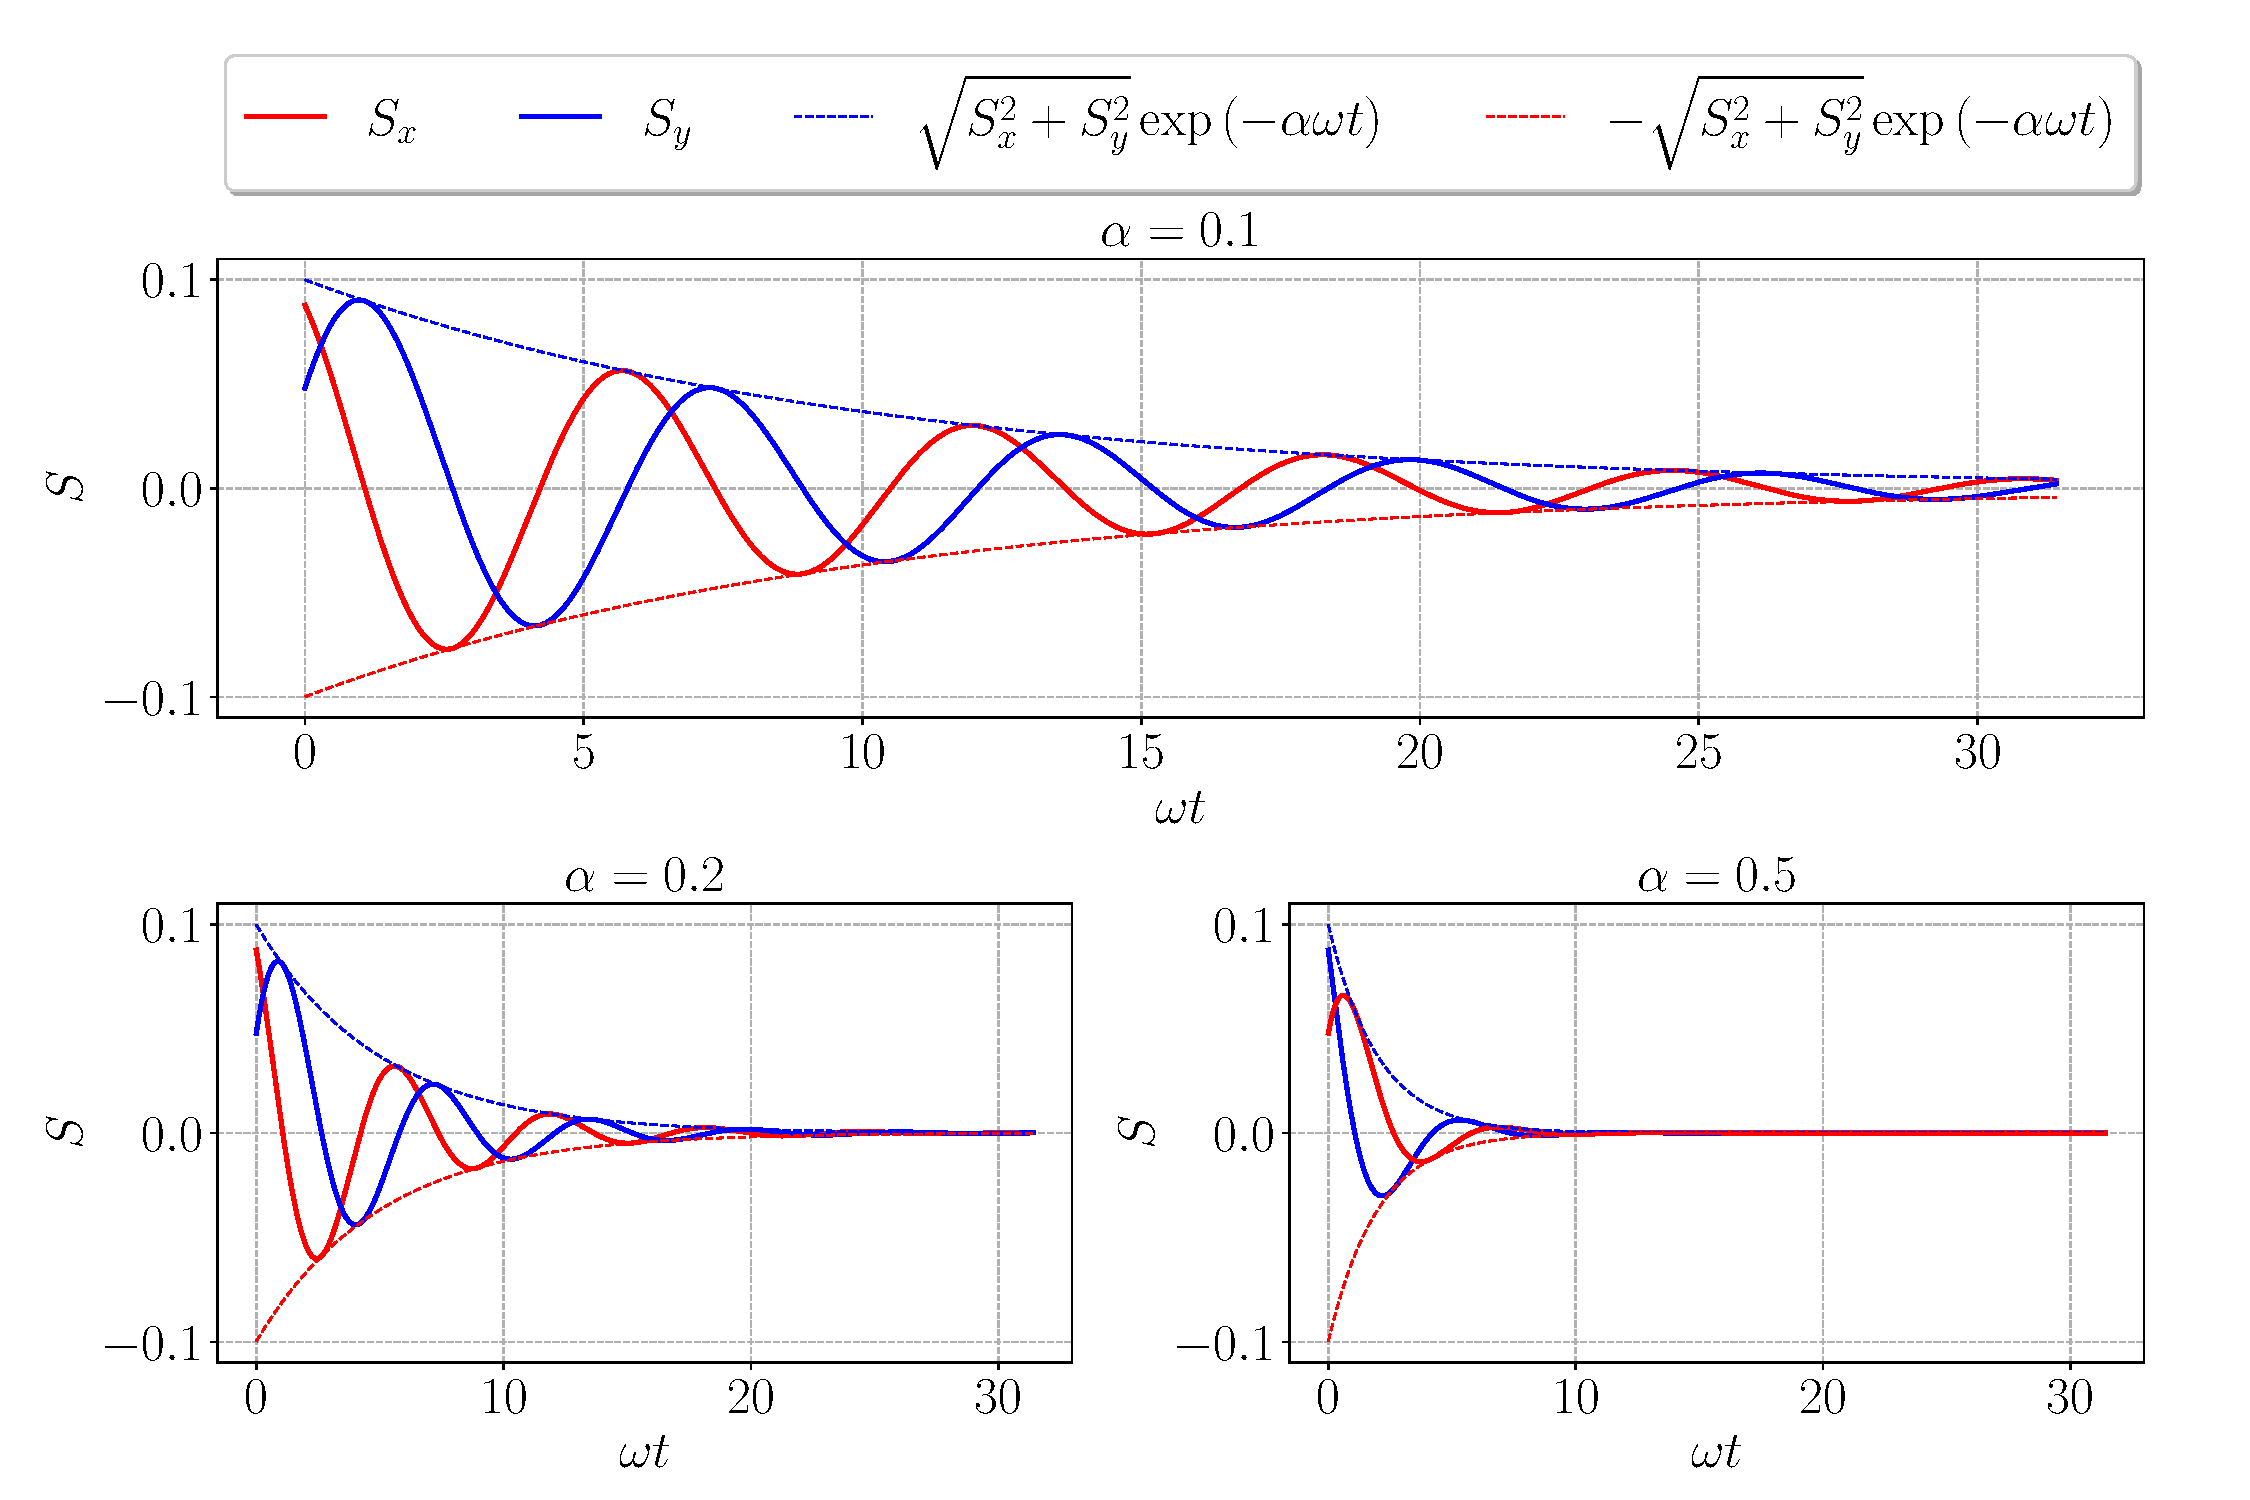
\includegraphics[width=\columnwidth]{../fig/damped_precession.pdf}
	\caption{Three different damped precessions.}
	\label{fig:damped}
\end{figure}